\documentclass[12pt]{article}
\usepackage{jeep}
\usepackage{unicode}
\usepackage{setspace}
\usepackage[scaled]{helvet}
\renewcommand\familydefault{\sfdefault}
\usepackage[T1]{fontenc}
\usepackage[numbers]{natbib}
\usepackage{tabularx}
\usepackage[hidelinks]{hyperref}
\hypersetup{
    colorlinks,
    citecolor=black,
    filecolor=black,
    linkcolor=black,
    urlcolor=black
}
\usepackage{float}
\usepackage{graphicx}
\usepackage{pdfpages}

\begin{document}
\linespread{1.0}
\begin{titlepage}
  \begin{center}
    \large{University of Puerto Rico\\
    Mayagüez Campus\\
    \vspace{\baselineskip}
    Department of Electrical and Computer Engineering\\}
    \vspace{6cm}
    \Huge{\underline{Insulin Temperature Warning System}\\}
    \vspace{0.5\baselineskip}
    \large by\\
    Fabio J. Matos Nieves\\
    Enrique Chompré\\
    Guillermo Colón\\
    Rubén Marrero\\
    \vspace{3.5cm}
    For: Professor Manuel Jimenez\\
    Course: INEL 4217 Seccion 096\\
    Date: Febuary 2, 2023\\
    \normalsize

  \end{center}
\end{titlepage}

\linespread{2.0}
\section*{Abstract}
The purpose of this document is outlining a design for a pair of devices that monitor the temperature of insulin, making sure that it meets the safe storage guidelines in a mass storage context. This document contains the system conception, system architecture \& functionality, specifications and market description as well as the project time table, design criteria and the opinion of the client of this design.

\tableofcontents
\newpage
\section{Introduction}
In 2017 hurricane Maria devastated the northeastern Caribbean, particularly Dominica, Saint Croix, and Puerto Rico. In the wake of the storm, Puerto Rico suffered the longest blackout in US history and the second longest blackout in recorded human history\cite{WorldSecondLargest}. The revised death count attributable to the hurricane was 2,975 people\cite{HurricaneMariaCaused2018}. According to an investigation by the New York Times, deaths caused by  sepsis, pneumonia, emphysema, diabetes, and Alzheimer's and Parkinson's spiked in the two months following the hurricane\cite{roblesOfficialTollPuerto2017}. The whole island of Puerto Rico was declared a disaster zone by the Federal Emergency Management Agency (FEMA) and it wasn't until four to eight months after the storm that most of the population had electricity and running water after the storm. The Puerto Rican electrical grid also collapsed in the aftermath of hurricane Fiona in September of 2022. Puerto Rico also has a sizable portion of the adult population with diabetes and a large portion of those diagnosed with diabetes require insulin to survive\cite{DiabetesPrevalencePopulation}. The rationale for this project is to provide a tool for users of insulin to be sure that their medication is safe and effective in normal and post-disaster conditions. The problem is that there has not been a way to monitor the storage conditions of insulin in a consumer setting in normal/post-disaster conditions. This project's solution to this problem is to create a micro-controller based design that can:
\begin{itemize}
  \item Monitor the temperature of the insulin.
  \item Check if a power-outage has occurred.
  \item Warn the main unit if the temperature has exceeded \textnormal{$15^{\circ}C$} and turn on a warning light on the sub unit.
  \item Record the temperature, time-stamp and power-availability on a log file on the main unit.
  \item Let the main unit warn an operator if a sub-unit has exceeded temperature guidelines.
  \item The main unit send its logging information to a device.
\end{itemize}

\section{System Conception}
\begin{figure}[H]
  \centering
  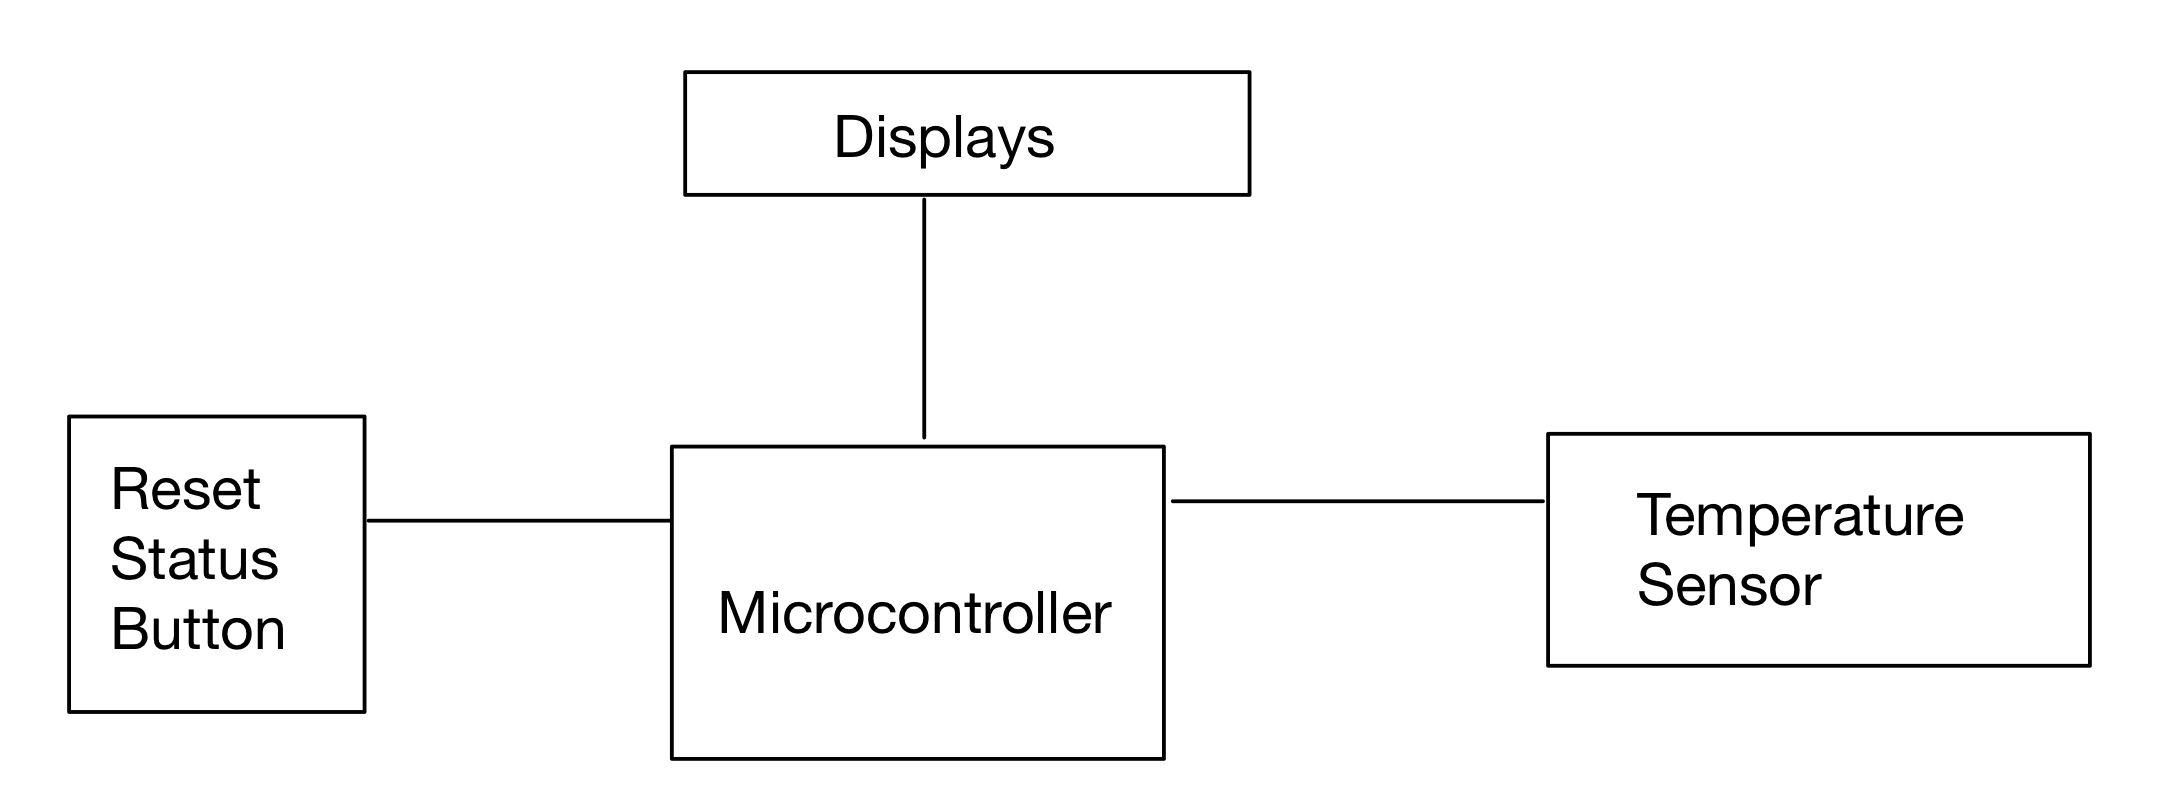
\includegraphics[width=\textwidth]{../System-Conception/Figures/global-system-view.png}
  \caption{Global System View}
\end{figure}
\begin{figure}[H]
  \centering
  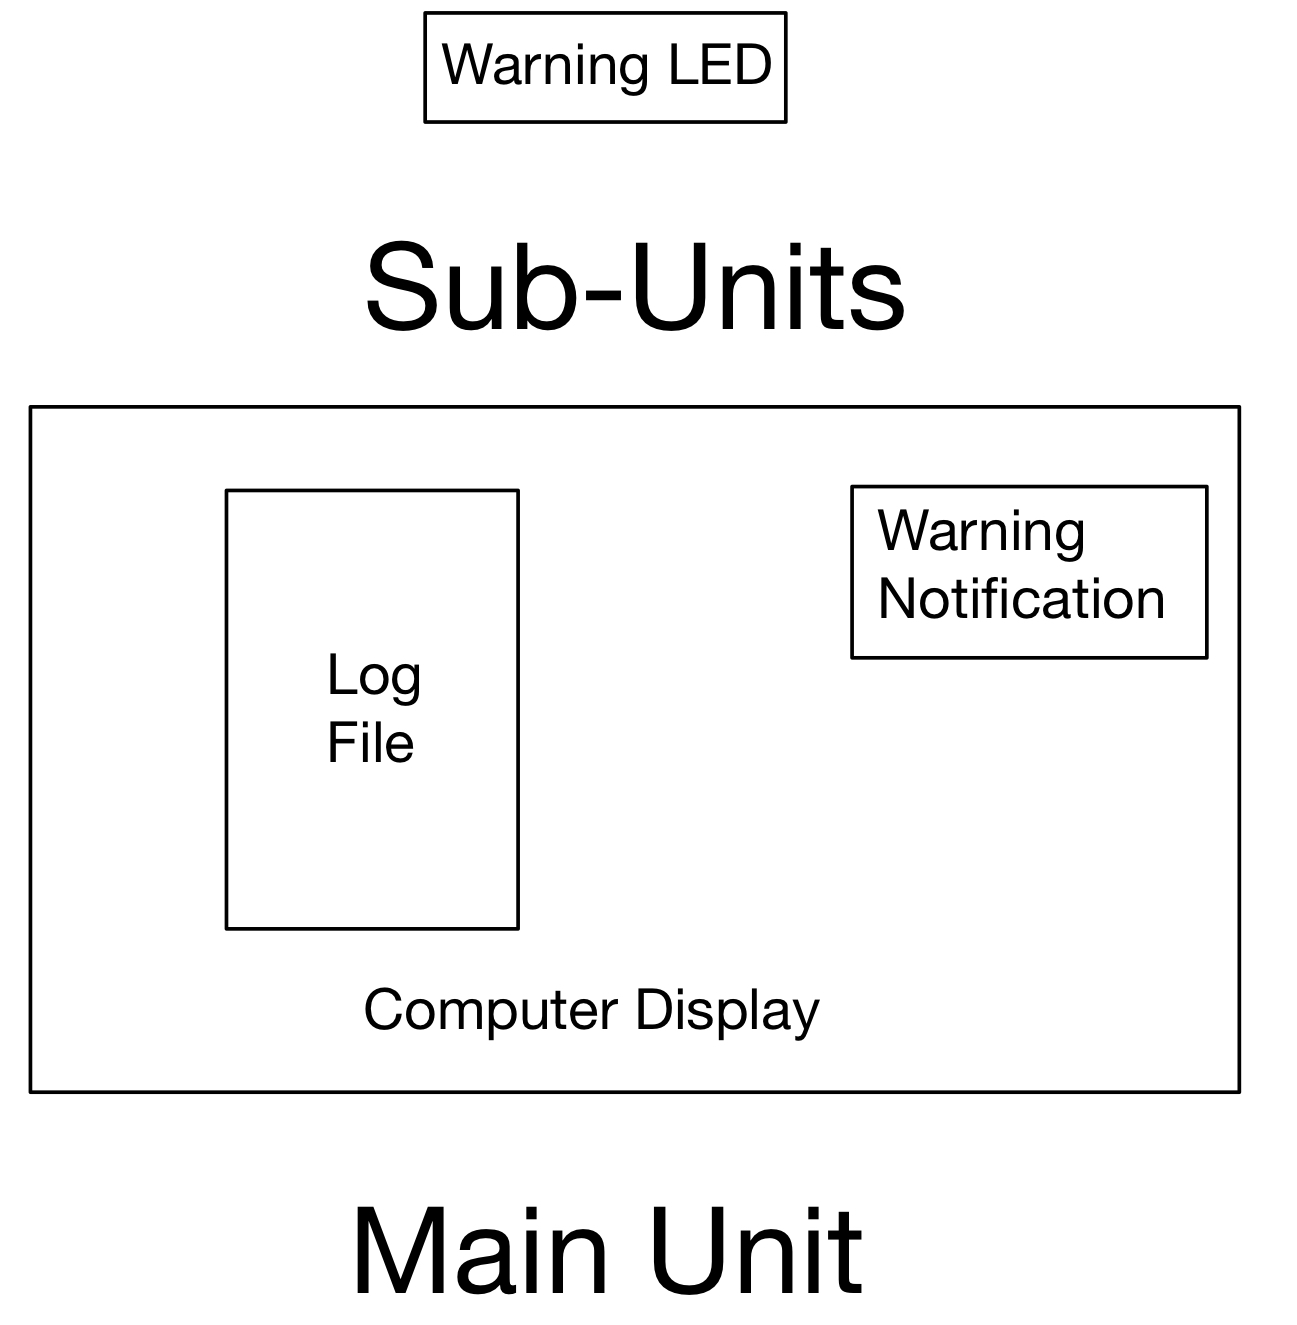
\includegraphics[width=\textwidth]{../System-Conception/Figures/user-interface-level.png}
  \caption{User Interface Level}
\end{figure}
\section{System Architecture and Functionality}
\begin{figure}[H]
  \centering
  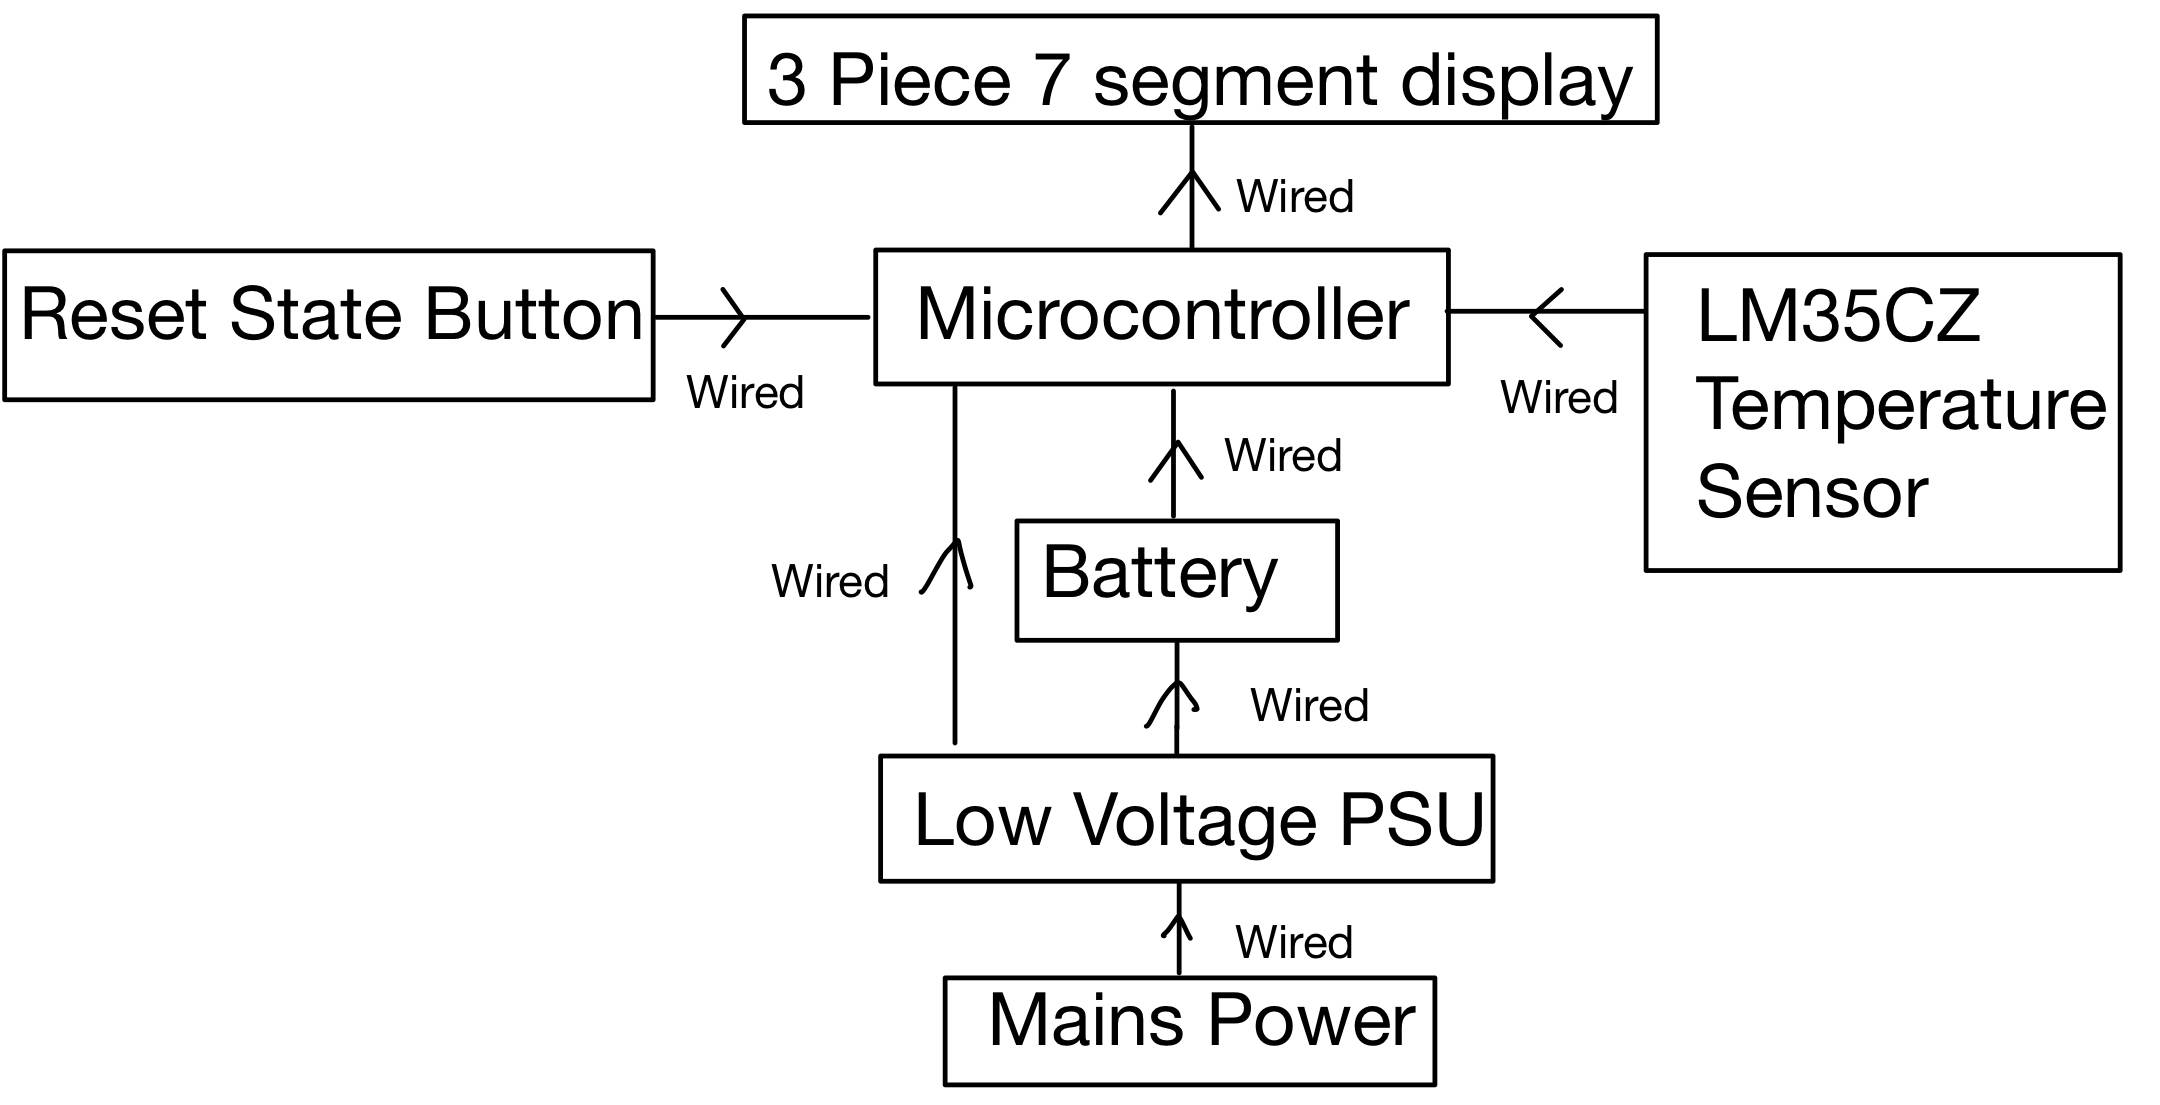
\includegraphics[width=\textwidth]{../System-Architecture-and-Functionality/Figures/system-architecture-block-diagram.png}
  \caption{System Architecture Block Diagram}
\end{figure}
\newpage
As shown above, this design will have two distinct units, the sub-units and a main unit.\\
\begin{enumerate}
  \item Sub\-Unit:
        \begin{itemize}
          \item Hold the current time and date, expiration date, and lot number.
          \item Check the current temperature.
          \item Verify if the temperature is meeting the guidelines.
          \item If the guidelines are not met, turn on an LED and send a warning
                to the main unit.
        \end{itemize}
  \item Main Unit:
        \begin{itemize}
          \item Receive error signals from the sub-units.
          \item Keep inventory of the lots.
          \item Send log files either periodically or on demand to an
                application.
          \item Send warning notifications to an application if an error has
                occurred.
        \end{itemize}
\end{enumerate}
The major software functions of this design will be:
\begin{itemize}
  \item Sub-Unit:
        \begin{itemize}
          \item Hold the current date and verify that is it less than the
                expiration date.
          \item If the current date is greater than expiration date, raise an
                error, send it to the main unit and turn on an LED.
          \item Verify that
                \textnormal{$2^{\circ}C < Current Temperature <= 8^{\circ}C$}.
                If not, turn on an LED and send a specific warning to the main
                unit following the current criteria.
                \begin{itemize}
                  \item \textnormal{$Current Temperature \leq 0^{\circ}C$}
                  \item
                        \textnormal{$0^{\circ}C < Current Temperature \leq 2^{\circ}C$}
                  \item
                        \textnormal{$8^{\circ}C < Current Temperature \leq 15^{\circ}C$}
                  \item \textnormal{$Current Temperature > 15^{\circ}C$}
                \end{itemize}
        \end{itemize}
\end{itemize}

\section{Processor Selection}
Based on the global system view, in terms of input output devices (I/O) the sub-unit just requires 1 Bluetooth module and an LED. A cursory glance on the internet reveals that a HC-05 Bluetooth module\cite{InterfacingHC05Bluetooth} uses two I/O and one I/O pin for controlling the LED. The main requires the same two pins for the Bluetooth module and one for detecting power outages. This means that both units need a measly three I/O pins and according to the HC-05 datasheet, the default baud rate is 38400 baud, which translate to 38.4 KHz which most MCU can easily obtain. There is no intense requirements for computation or memory, but peripherals are required, thus it is justified that an MCU be used for this design. However, the MCU has to be very low power since the sub-units only operate on batteries and have to last at least a year due to the fact that refrigerated vials of insulin can last upwards of
\begin{enumerate}
  \item MSP430F5515IPN: It has 63 I/O, a real time clock (RTC) and 12 bit ADC with a unit price of \$5.50. It also has a development kit and IDE for rapid prototyping.
  \item STM32F100RCT6B: It has 51 I/O, also has an RTC and a 12 bit ADC with a unit price of \$7.59. It also has an IDE, official libraries and development kit similar in price to the MSP430 but with a unit price almost 50\% more expensive than the MSP430.
  \item PIC24FJ256GA106-I/PT: It has 64 I/O, also has an RTC, a 16 bit ADC with a unit price of \$7.57. It also has a development kit and IDE but the development kit is almost three times more expensive than the MSP430 and per unit price it is almost 50\% more expensive.
\end{enumerate}
With this design being focued on low cost due to mass production, the MSP430F5515IPN was chosen due to it's lowest price per unit, IDE and development kit availability.

\section{Specifications}
The major requirements, features and limitations for hardware and software for this design are as follows:
\begin{itemize}
  \item Sub-Unit:
        \begin{itemize}
          \item Hold the current time, expiration date and lot number in memory.
          \item Check the current temperature using the on-board temperature sensor.
          \item Check that the current temperature meets safe storage guidelines.
          \item Check that the current time is less than the expiration date
          \item Send an appropriate error code if either expiration date has been passed or the current temperature is not within the guidelines.
                \item Send lot number information to the main-unit.
        \end{itemize}
  \item Main-Unit:
        \begin{itemize}
          \item Check that the current temperature meets safety guidelines for safe storage.
          \item Receive error codes from the sub-units.
          \item Forward error codes to an application that an operator can take appropriate action on.
          \item Check if mains power is available.
          \item Log the current temperature power, status and time to a log file and periodically forward it to a server.
          \item Alert an operator via an app if the temperature does not meet the safety guidelines or that power is not available.
          \item Send logs of lots of sub-units that entered the main-units range.
        \end{itemize}
\end{itemize}
This design satisfies all four essential component for eligibility as follows:
\begin{enumerate}
  \item \underline{Communications}: This design communicates 2 ways:
        \begin{itemize}
               \item The sub-units sends their lot numbers to the main-unit once they are in range and the main-unit forwards that information to a server.
               \item The sub-units send error codes to the main-unit and then the main unit sends the error information to an application where an operator can take further action based on the information provided.
        \end{itemize}
  \item \underline{User Interface}: For the sub-units the only way that it interacts with a user is via an LED, warning the user if an error status has occurred. The main unit, interacts with a user via the sent logs being displayed by an app and warning notifications if a critical error has occured.
  \item \underline{Control Scheme}: The main way that this design controls something, is that it notifies an operator to take action if a sub-unit sends an error and then can take appropriate action the box on insulin.
  \item \underline{Microprocessor-based}: This design meets the needs for it to be microprocessor based in that we need the sub-units to be low cost, and exceedingly power efficient without needing access to a lot of RAM or storage but still needing to have I/O. The main unit also necessitates it based due to not having to compute much, needing to have I/O and relatively low requirements for memory and storage and needing it being inexpensive.
\end{enumerate}

\section{Market Description}
The market target of our system is the Fridge-tag® 2 L with a serial number of 51050000XXXX \cite{RefrigeratorTemperatureMonitoring}. This device is similar to the idea of our project, is a high precision temperature data logger but it focuses on the monitoring of sensitive vaccines and pharmaceuticals stored in medical refrigerators \& freezers. The Fridge-tag 2 L automatically triggers an alarm when a critical temperature deviation out of the predefined temperature range is measured. This enables to react just in time and avoid serious quality issues while complying to various regulations.
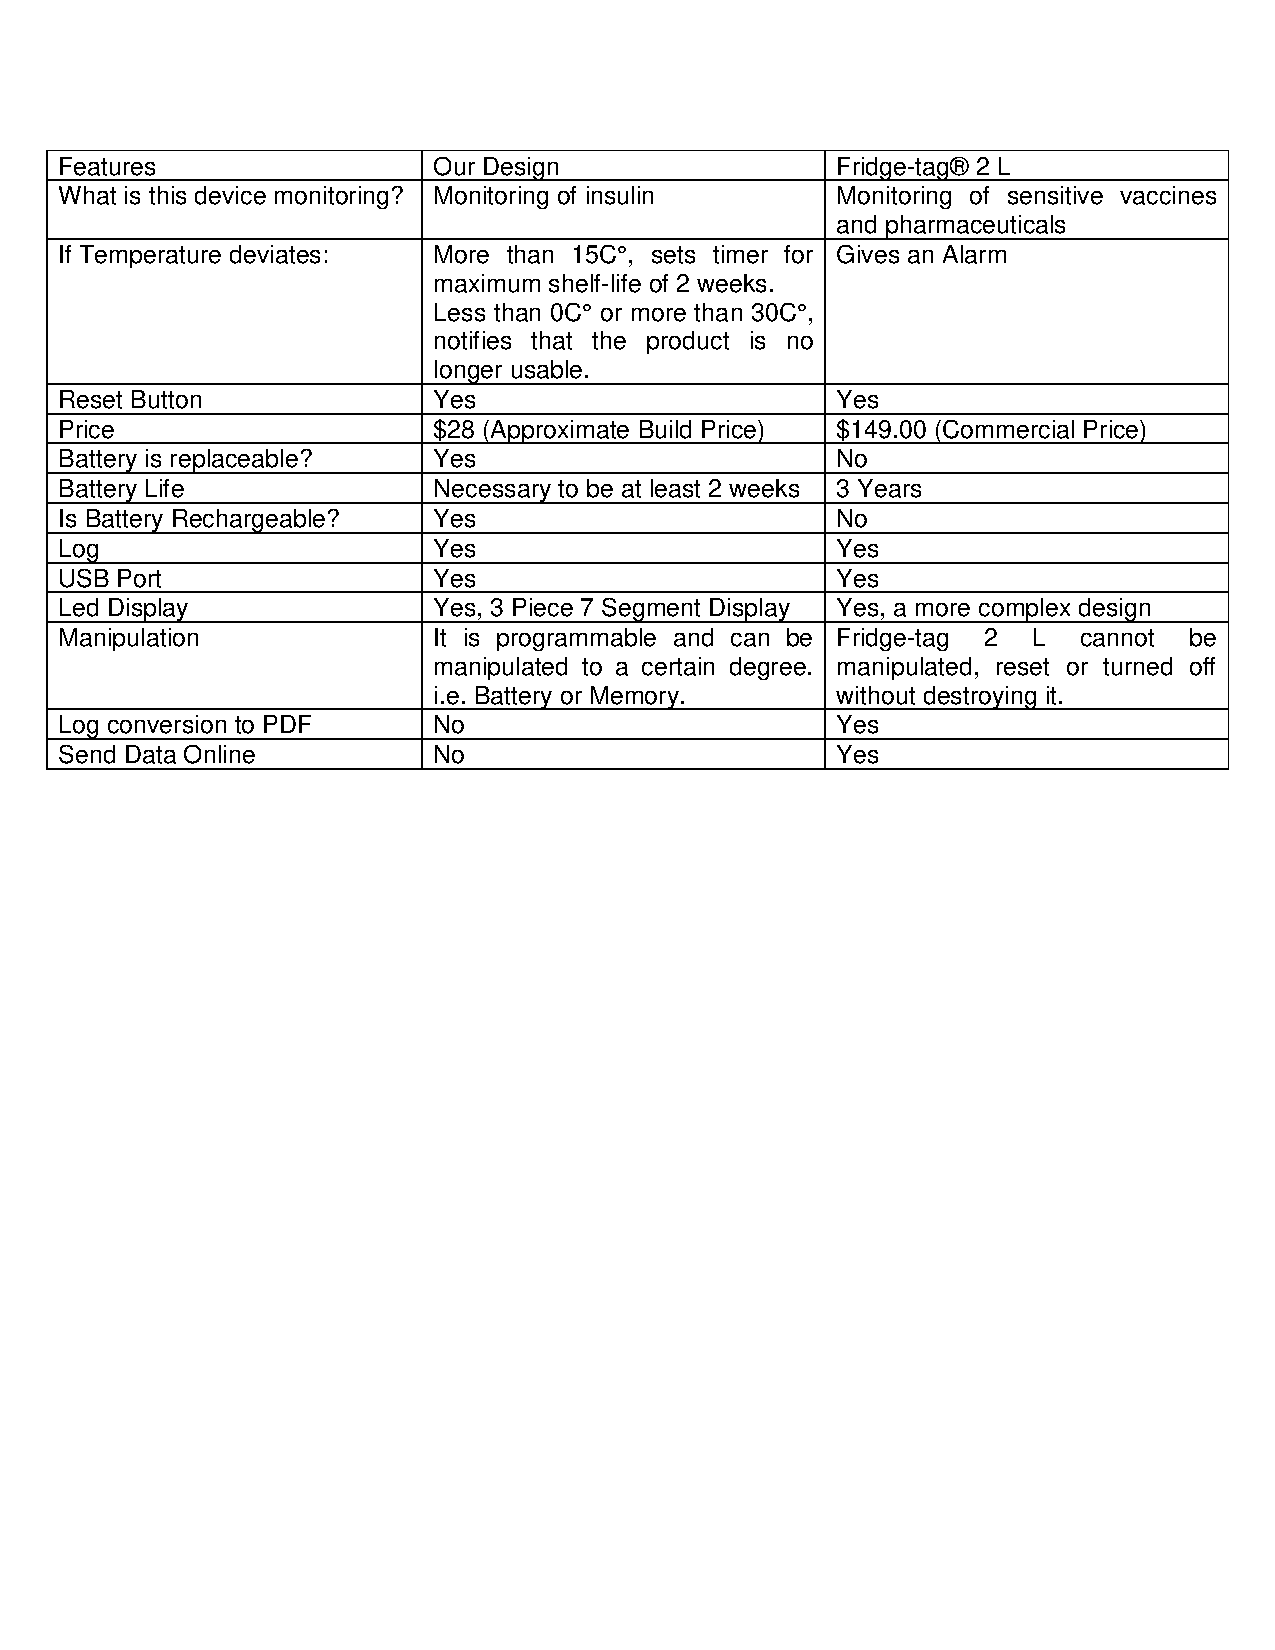
\includepdf[pages=-]{../Market-Description/market-description.pdf}
As seen in this table where we are comparing both devices, one noticeable aspect is the battery. While ours is replicable and chargeable, Fridge-tag® 2 L's Battery is not and after 3 years a new device needs to replace the previous one, forcing the user to buy new devices every 3 years for the price of \$149.00. Other aspect is the display used to give the user any logs / data available. Our design will use an application that will display the log / data via Bluetooth while Fridge-tag® 2 L is using a custom LCD display. Like we previously said, our design specializes in the monitoring of insulin but this other product specializes in a variety of meds and vaccines that are temperature sensitive. A few examples are ALL vaccines, Victoza, Botox, Humira, Byetta and Caverject. Finally, one critical factor is that our design will be able to transfer data / log converted to PDF via Bluetooth using an app while this other design uses a USB port. Regarding logging and expiration dates in our design, it will be the responsibility of the main unit. 
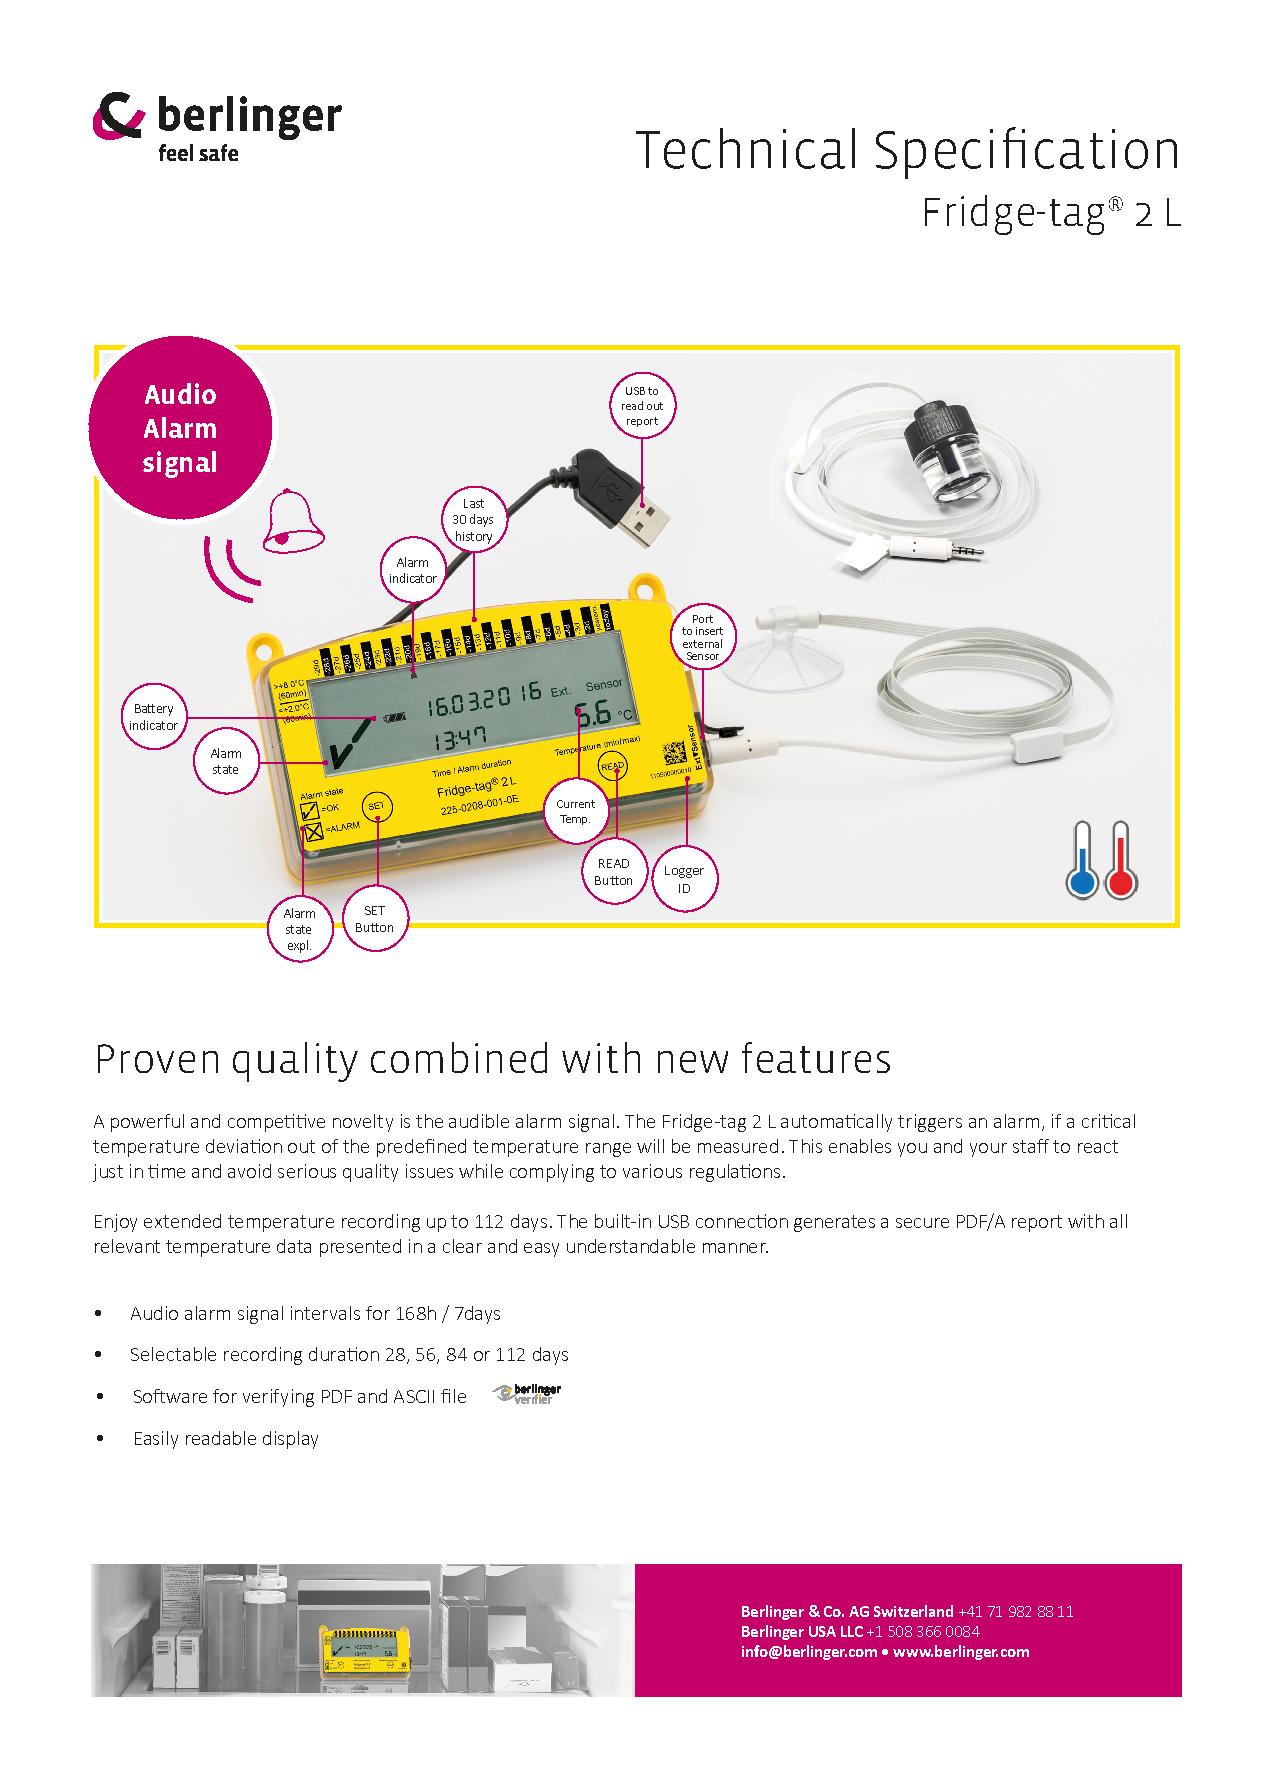
\includepdf[pages=-]{../Market-Description/documentation.pdf}

The market target of our system is the Fridge-tag® 2 L. This device is similar to the idea of our project, is a high precision temperature data logger but it focuses on the monitoring of sensitive vaccines and pharmaceuticals stored in medical refrigerators \& freezers. The Fridge-tag 2 L automatically triggers an alarm when a critical temperature deviation out of the predefined temperature range is measured. This enables to react just in time and avoid serious quality issues while complying to various regulations.
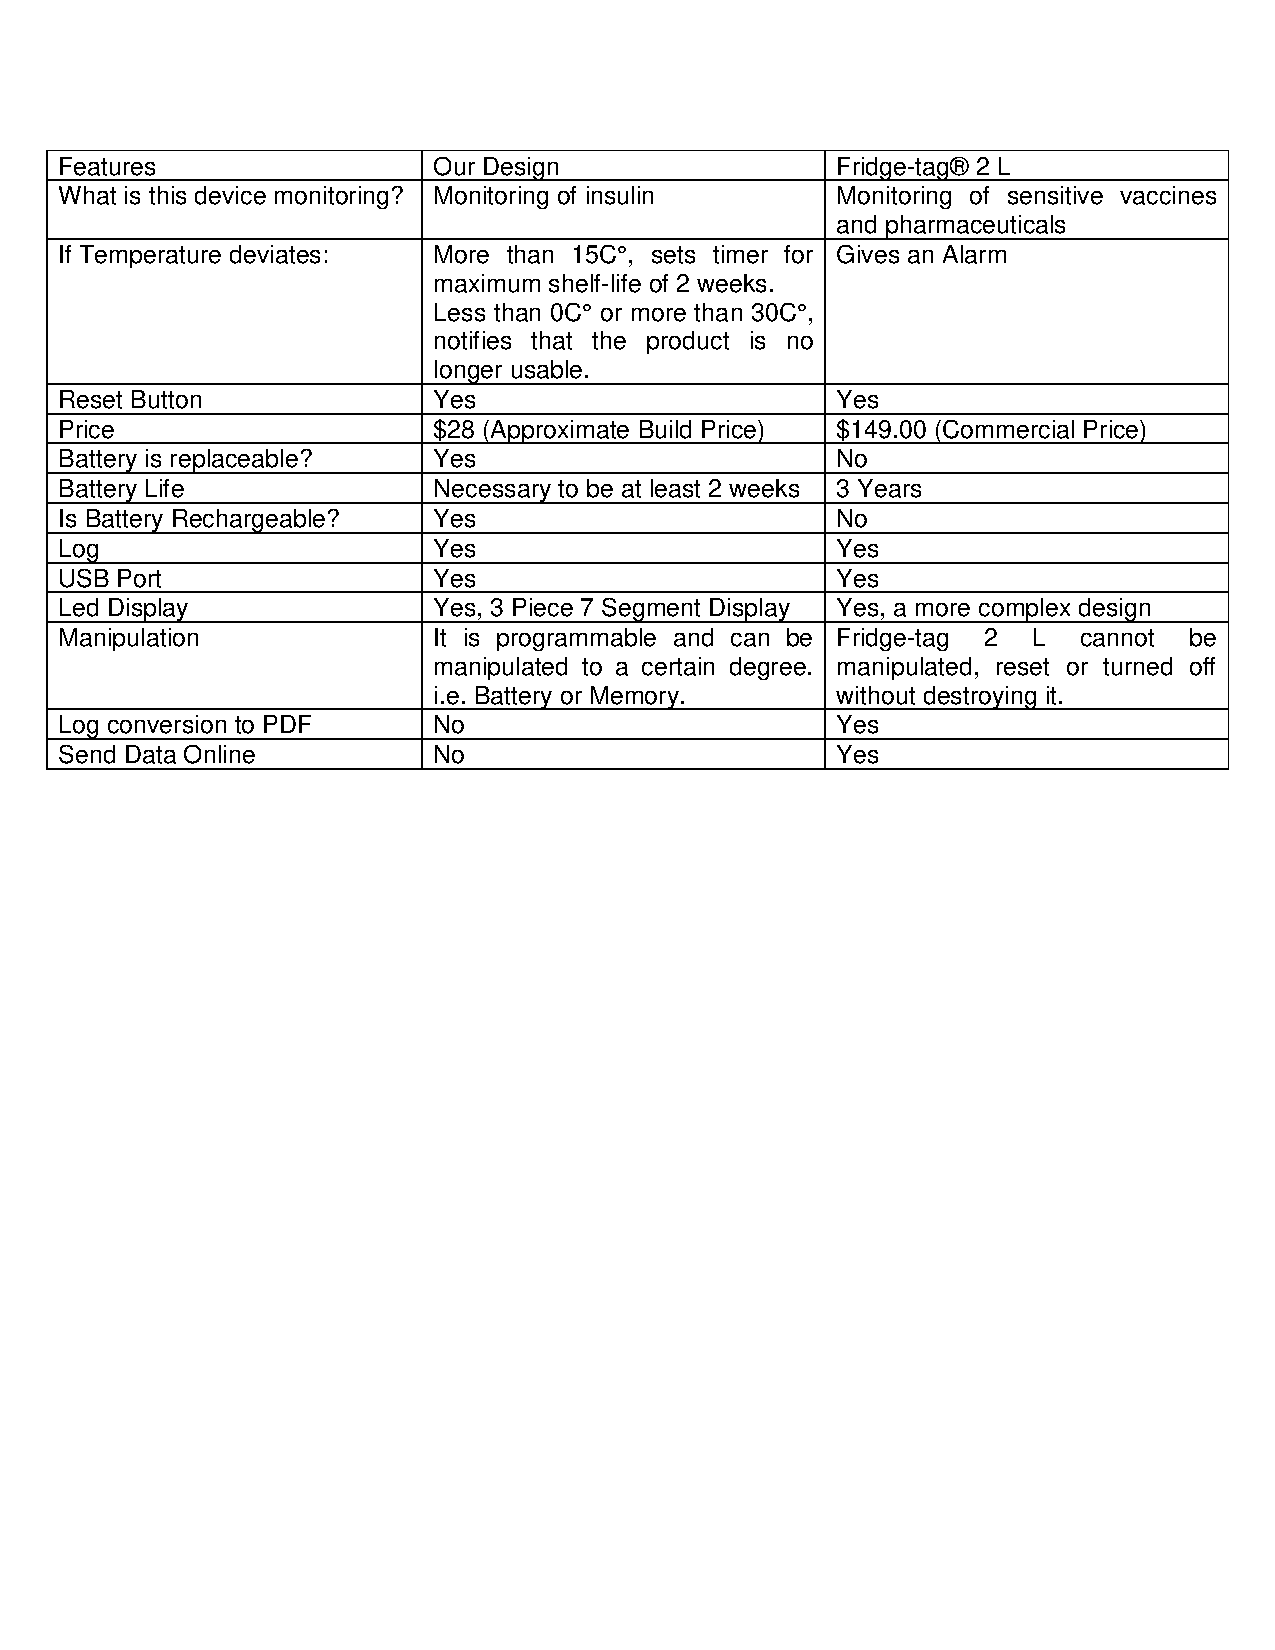
\includepdf[pages=-]{../Market-Description/market-description.pdf}
As seen in this table where we are comparing both devices, one noticeable aspect is the battery. While ours is replicable and chargeable, Fridge-tag® 2 L's Battery is not and after 3 years a new device needs to replace the previous one, forcing the user to buy new devices every 3 years for the price of \$149.00. Other aspect is the complexity of the LED display. Ours is a simple 3 Piece 7 Segment Display while Fridge-tag® 2 L's display is a more complex design. Another factor is that our design has no need to transfer data online considering that this design will be usable for situation where we don't have internet connection due blackouts.
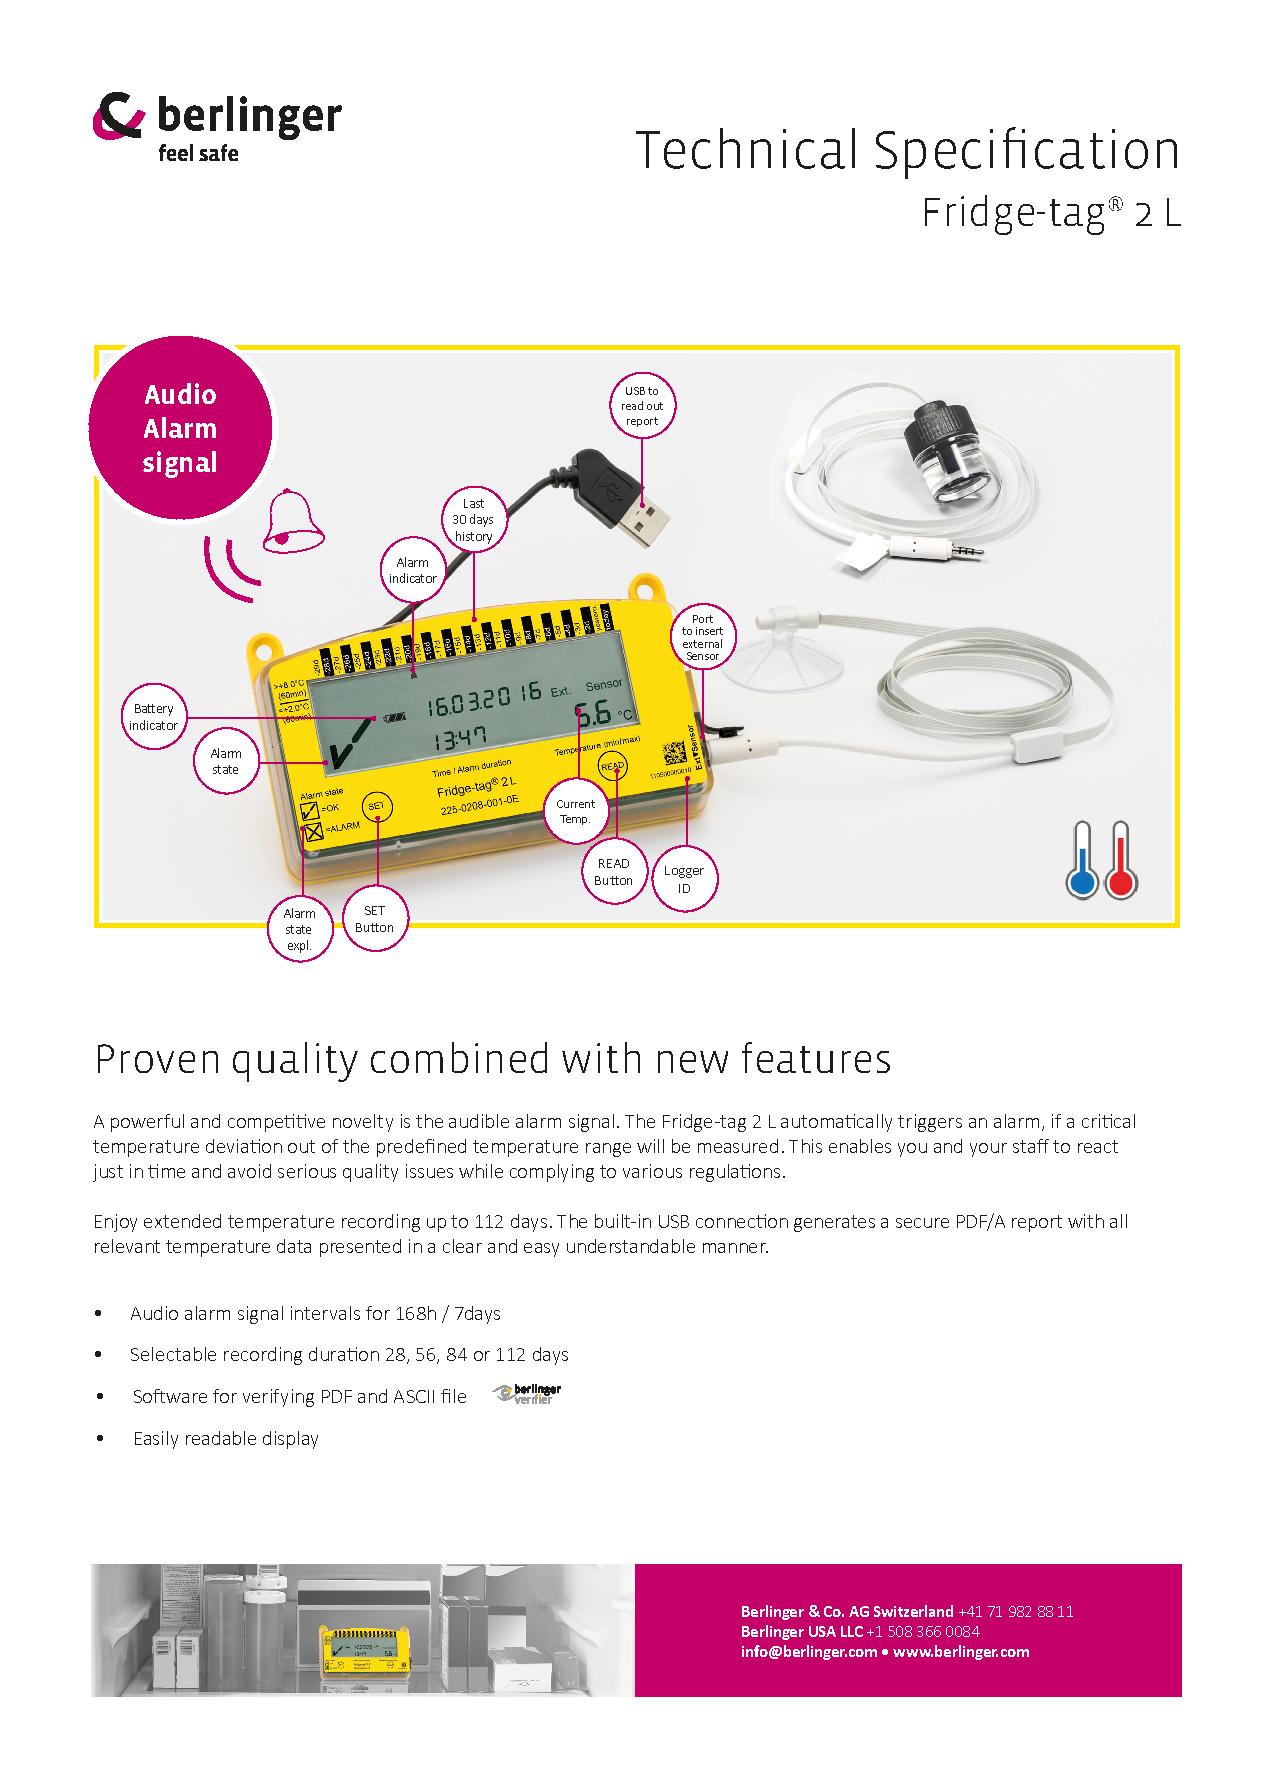
\includepdf[pages=-]{../Market-Description/documentation.pdf}
\section{Design Criteria}
\begin{enumerate}
  \item Economic: This design is supposed to be inexpensive enough so that insulin patients can afford it when purchasing their first batch of insulin or as an accessory that can be purchased at a pharmacy.
  \item Power/Energy: The crux of this design is to be able to operate in conditions where the mains power has been disabled by a natural disaster for weeks.
  \item Manufacturability: This design used of the shelf parts that are in actively being manufactured and are easy to assemble.
\end{enumerate}

\section{Project Time Table}
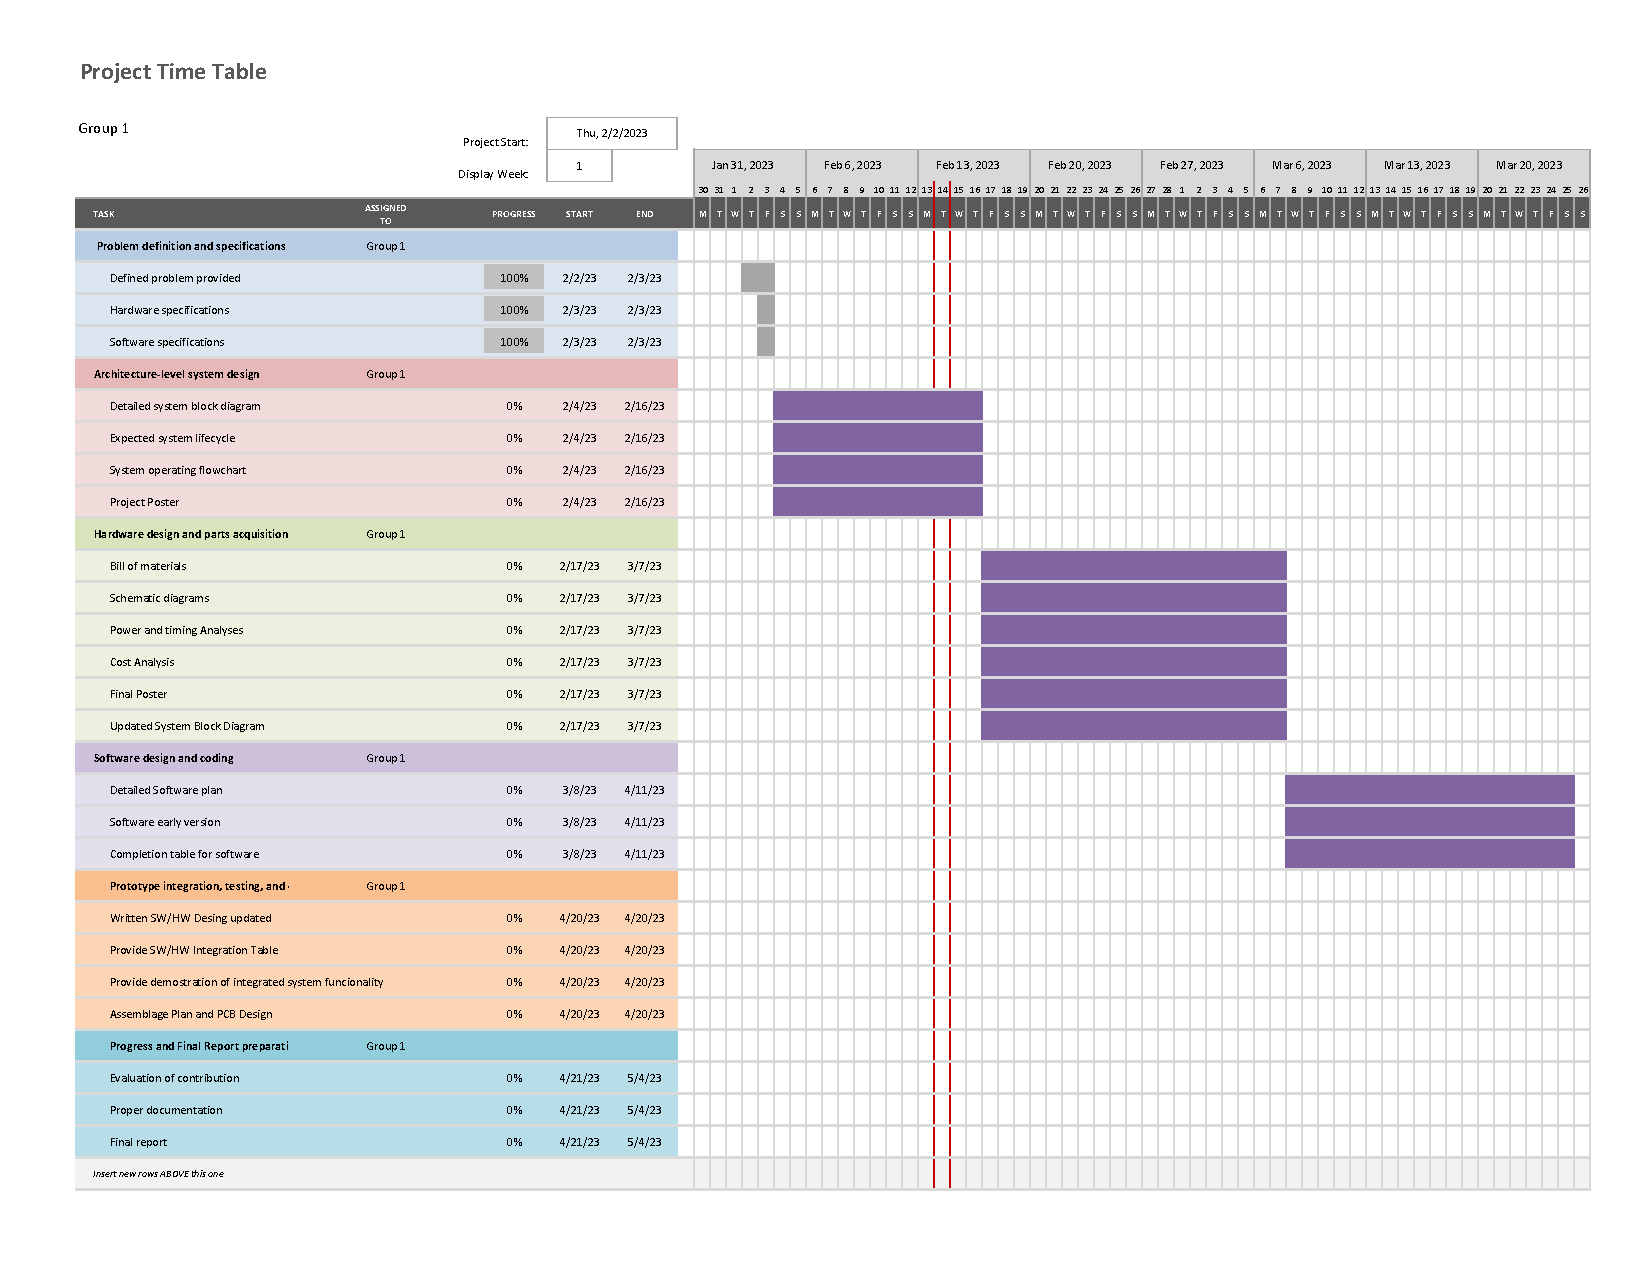
\includepdf[pages=-]{../Project-Time-Table/project-time-table.pdf}

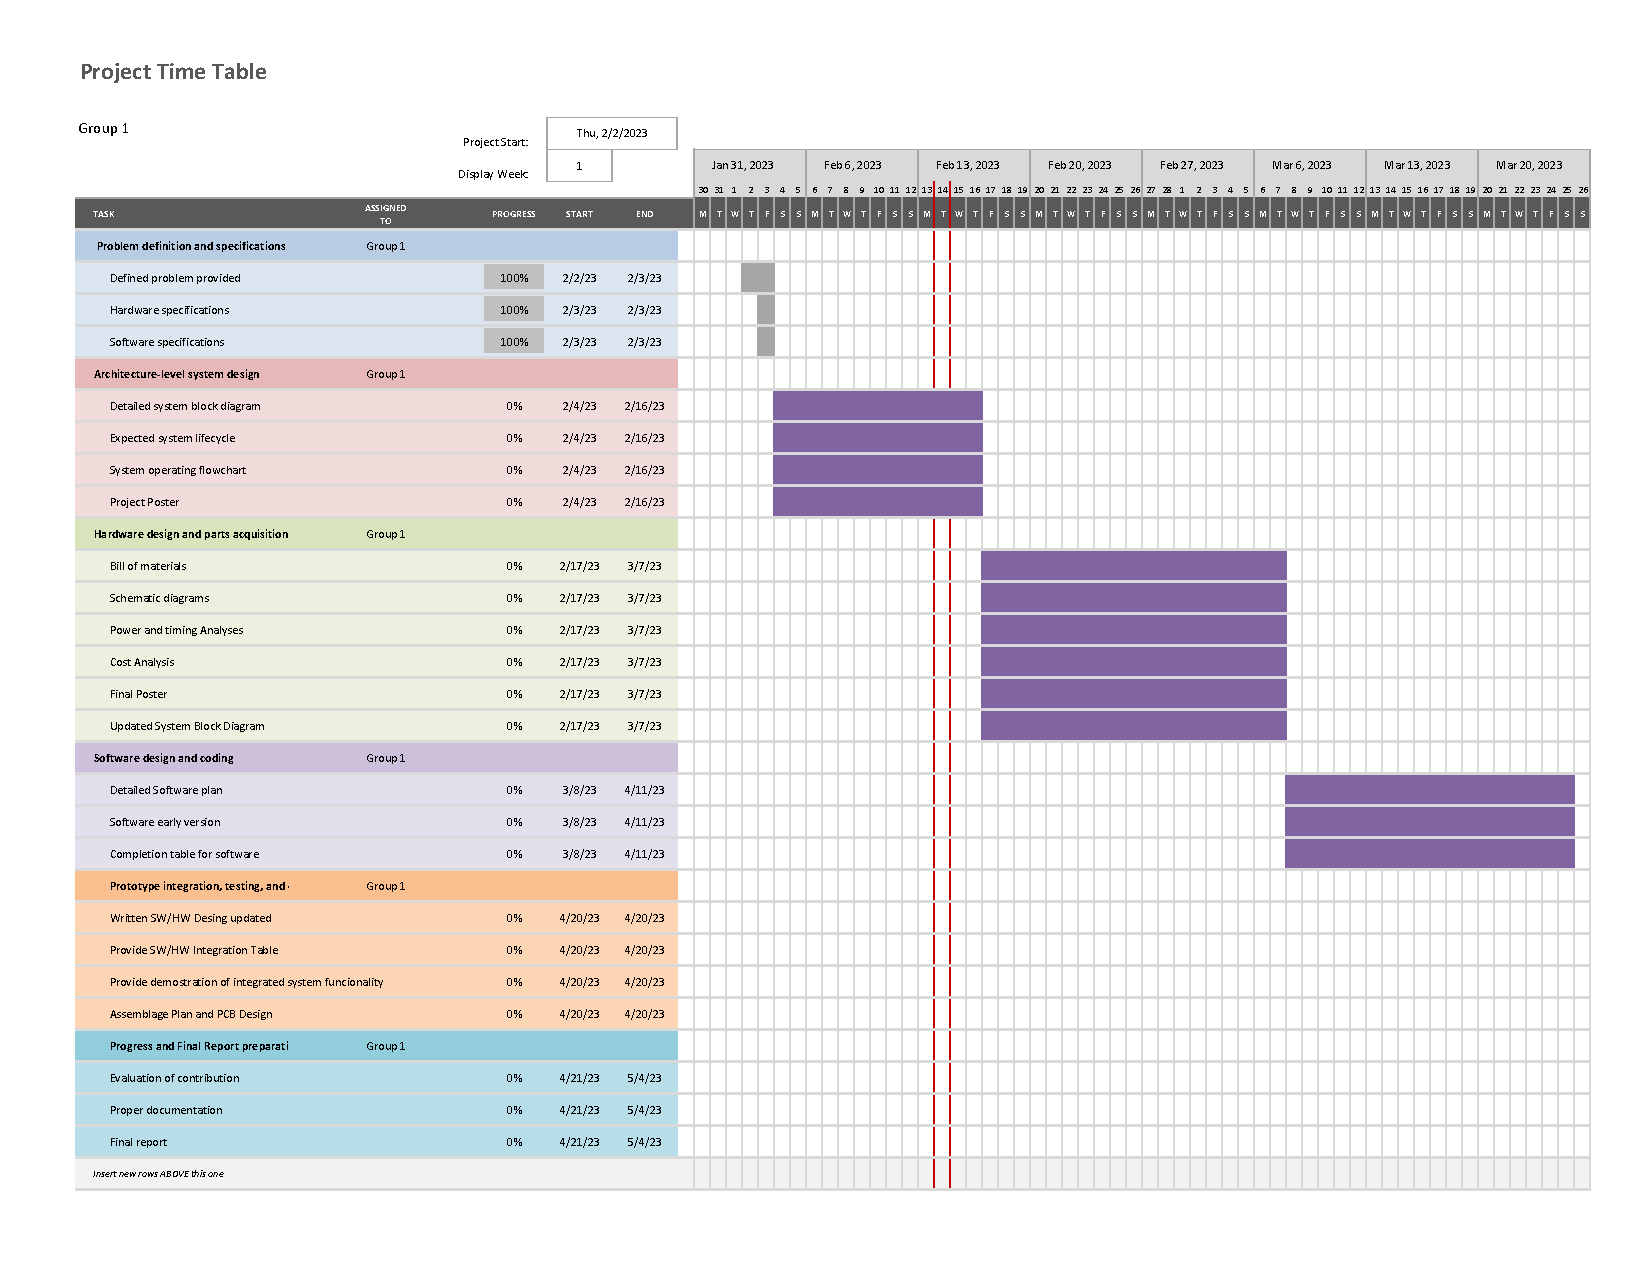
\includepdf[pages=-]{../Project-Time-Table/project-time-table.pdf}
\chapter{Client Opinion}

\bibliographystyle{IEEEtranN}
\bibliography{../References/Proposal-Biliography}
\section{Appendices}
\begin{figure}[H]
  \centering
  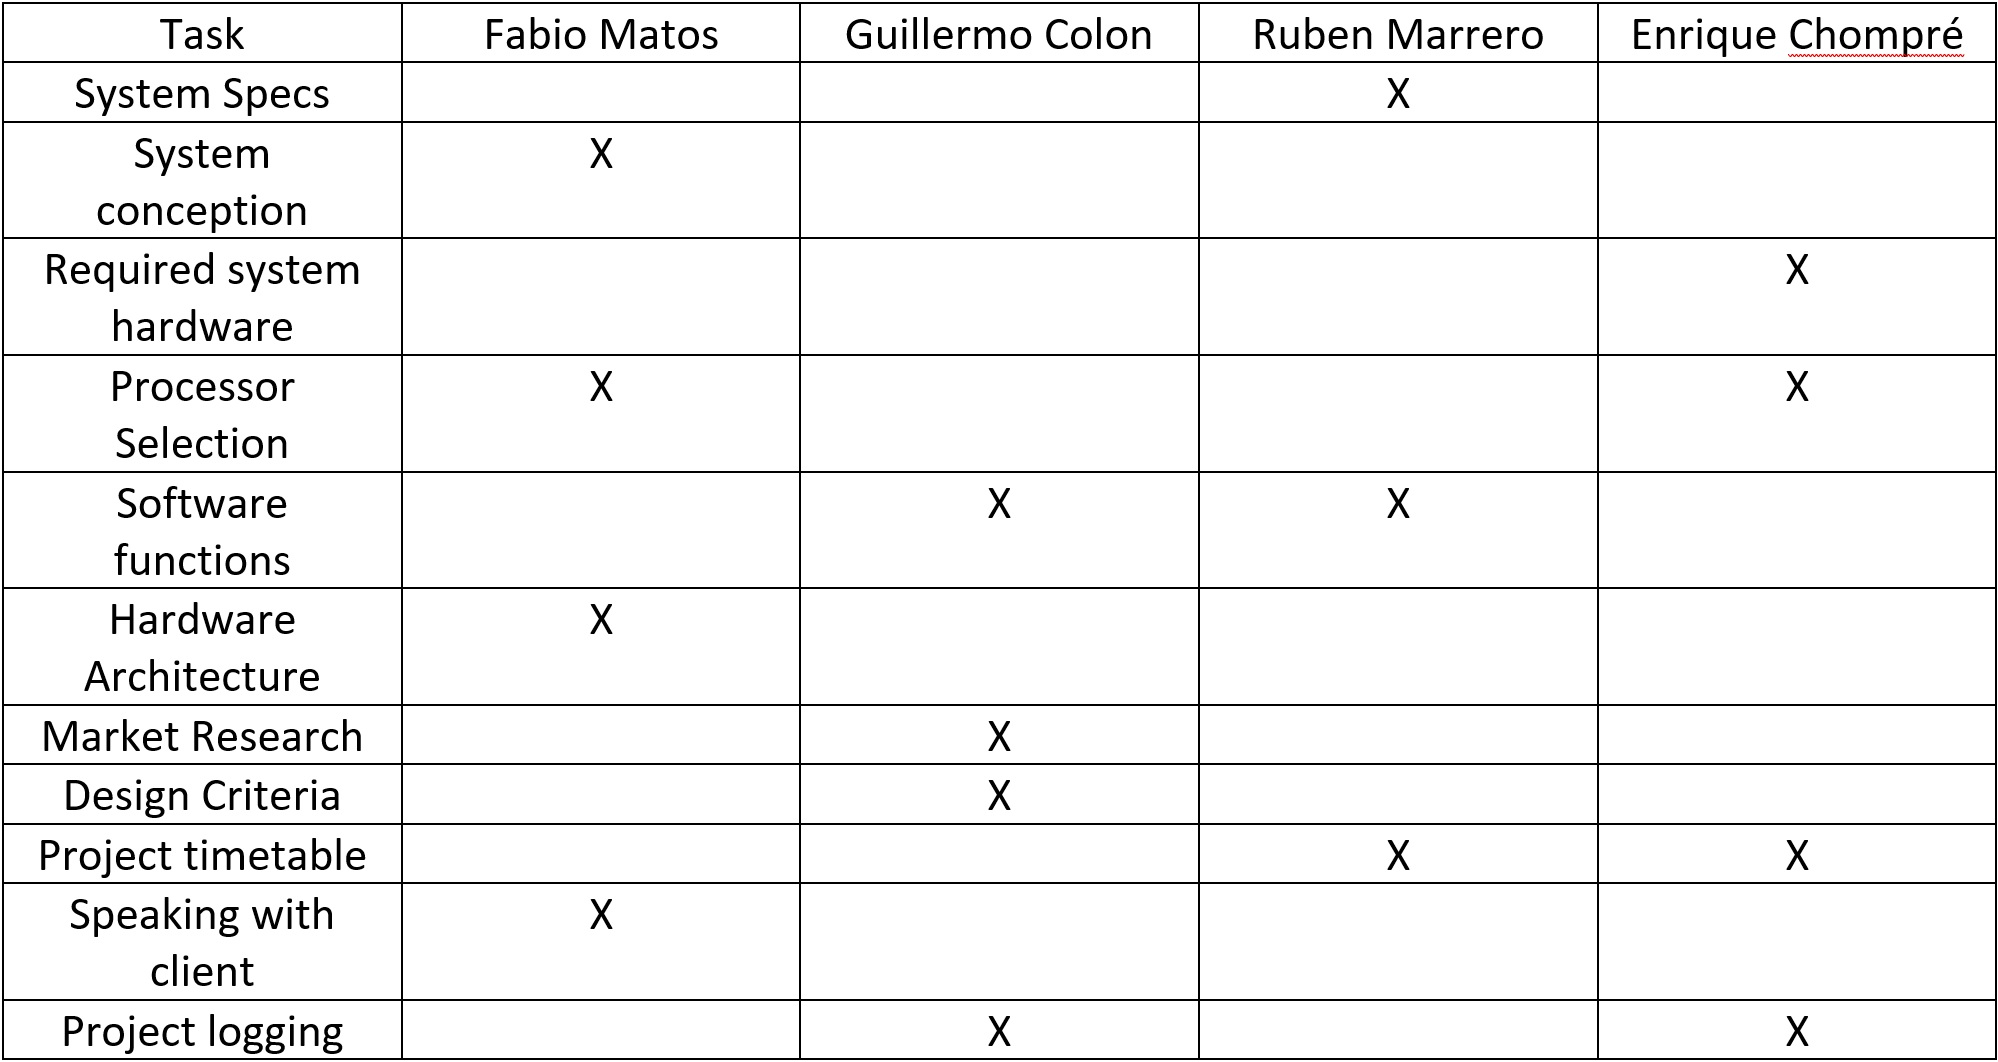
\includegraphics[width=\textwidth]{../Appendices/Figures/work-distrobution-table.jpeg}
  \caption{Work Distribution Table}
\end{figure}
Work Distribution Table

Project Journal 
January 21, 2023 at 3:00pm: First team meeting where all members where present. Discussed initial proposal ideas, potential clients and started work on pre-proposals to be sent for review.

January 28, 2023 at 1:00pm: Team meeting with all team members present. Team leader fixed their proposal while other team members searched for new ideas with new clients. Discussed several ideas and reached new ideas and new clients where the rest of the team members continued to develop. Also ranked all ideas and provided details for each proposal. Also started work on proposal document to be sent. Each team member assigned a part to do once an idea was selected after pre-proposal review. 

January 29, 2023 at 6:00pm: Small meeting between team leader Fabio Matos and team member Enrique Chompré. Discussed new idea for proposal and new client. Finished new pre-proposal document for review.

\end{document}
